\scanpage{46}
\mspage{2}
\uline{objets} : Triples $(X,\widetilde\Sigma,
\deleted{\unsure{S}}\inserted{R})$, \unsure{où|ou}

$X$ surface à bord compacte orientée

$\widetilde\Sigma$ sous-variété compacte de $X$
\deleted{\unsure{close}}, $\widetilde\Sigma\supset\partial X$


\begin{tikzpicture}[x=.13cm,y=.13cm,baseline=-.1ex,line width=.5pt]
\draw (.08,.05) .. controls (-.03,.42) and (.24,.67) .. (.62,.89)
 .. controls (.97,.97) and (1.02,.7) .. (.72,.48)
 .. controls (.47,.28) and (.3,.08) .. (.08,.05);
\draw (.12,.15)--(.81,1.08);
\draw (.32,.04)--(.98,.78);
\draw (.11,.62)--(.83,.13);
\end{tikzpicture}
$\deleted{\unsure{S}}R\subset\Sigma\deleted{\unsure{\widetilde\Sigma}}$,
partie finie

\margin{$X,\deleted{\partial X},\Sigma,S$}
\margin{$\widetilde\Sigma=\partial X\amalg\Sigma$

On peut considérer que $R$ rigidifie, \unsure{mais} aussi $\widetilde\Sigma$\ldots{}
que $R$ ``découpe''}

\uline{flèches} : classes d'isotopie d'homéom. conservant l'orientation

\deleted{Variante \unsure{de}}
Les compos. connexes de $\widetilde\Sigma\setminus\partial X
\inserted{=\Sigma}$ sont les \uline{cercles de découpage},
\inserted{celles de $\partial X$ sont les cercles de raccord},
les éléments de $\deleted{\unsure{S}}R$ sont les
\deleted{\unsure{pts de marquage}} \uline{sommets de}
\deleted{\uline{marquage}}\inserted{rigidification},
\deleted{(ou de rigidification)},
\deleted{les \unsure{composantes} connexes de $\partial X$ sont les ``\uline{trous}''}.
Les composantes connexes de $X$ sont les
\deleted{connexes}\inserted{\uline{composants}}
de l'objet envisagé.

Variante $S_*\mathcal TD_{\mathrm{top}}^\pm$, avec
\diagram{\begin{tikzcd}[ampersand replacement=\&,column sep=large]
S_*\mathcal TD_{\mathrm{top}}
\arrow[r,phantom,"{
\begin{tikzpicture}[x=1cm,y=1cm,baseline=-.15ex]
\draw (.23,.16) .. controls (-.05,.16) and (-.08,-.02) .. (.15,-.02)--(1.15,.02);
\end{tikzpicture}}" description]\&
S_*\mathcal TD_{\mathrm{top}}^\pm\arrow[r]\&{[\pm1]}
\end{tikzcd}}
comme tantôt.

On a des sous-groupoïdes pleins
\diagram{\(\begin{array}{ccl}
R=\varnothing,\ \Sigma=\unsure{\varnothing}&
\mathcal T_{\mathrm{top}}\quad\text{et}\quad\mathcal T^\pm_{\mathrm{top}}&\\
\deleted{\unsure{R=\widetilde\Sigma=\varnothing}}&&\\
\Sigma=\deleted{\unsure{\partial X}}\unsure{\partial X|\varnothing\deleted{X}}&
S_*\mathcal T_{\mathrm{top}}\quad\text{et}\quad S_*\mathcal T^\pm_{\mathrm{top}}&
\begin{gathered}
\text{(groupoïdes de Teich-}\\
\text{müller \uline{spéciaux}}\\[-.1ex]
\text{\inserted{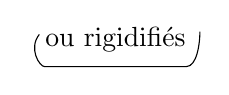
\begin{tikzpicture}[baseline=(rig.base)]
\node[anchor=base west,inner sep=0pt] (rig) at (0,0) {ou \uline{rigidifiés}};
\draw ([xshift=-2pt,yshift=2pt]rig.west)
 .. controls ([xshift=-6pt,yshift=-3pt]rig.west) and ([xshift=-2pt,yshift=-5pt]rig.south west) .. ([yshift=-5pt]rig.south west)
 --([yshift=-5pt]rig.south east)
 .. controls ([xshift=4pt,yshift=-5pt]rig.south east) and ([xshift=5pt,yshift=-1pt]rig.east) .. ([xshift=5pt,yshift=3pt]rig.east);
\end{tikzpicture}}}\\
\text{(topologiques orientés)}
\end{gathered}\\
R\text{ quelconque}&&\\
R=\varnothing&
\mathcal T_{\deleted{\unsure{\mathrm{top}}}}D_{\mathrm{top}}\quad\text{et}\quad\mathcal TD^\pm_{\mathrm{top}}&
\end{array}\)}
(Cas pas intéressant je crois, sauf pour $\Sigma=\unsure{\varnothing}$
également)

\margin{MD = ``modulaire'' ou \unsure{Mumford}--Deligne}

\deleted{\unsure{Dé}} \uline{Détermination} du
$\pi_0(S_*\mathcal TD_{\mathrm{top}})
 \xrightarrow{\sim}\pi_0(S_*\mathcal TD^\pm_{\mathrm{top}})$.

On introduit les \uline{graphes} \deleted{\unsure{MD}} bipondérés
\margin{45}
